% !TEX root = ../notes_unsupervisedlearning.tex
% Chapter 10: Weak Supervision and Labeling Functions
%%%%%%%%%%%%%%%%%%%%%%%%%%%%%%%%%%%%%%%%%%%%%%%%%%%%%%%%%%%%%%%%%%%%%%

\chapter{Weak Supervision and Labeling Functions}\index{Weak Supervision}\index{Snorkel}
\newthought{What if labels are noisy, partial, or heuristic?}

%═══════════════════════════════════════════════════════════════════════
% BLOCK 1: INTRODUCTION
%═══════════════════════════════════════════════════════════════════════

\section{The Why}

\marginnote{Labels are random variables, not ground truth facts.}

The assumption of clean labels is a fiction: crowd workers make mistakes with 5--20\% error rates, experts disagree on ambiguous cases, heuristics provide cheap but noisy labels, and legacy data carries inconsistent labelling standards.

\newthought{Rather than pretend labels are perfect,} weak supervision\index{weak supervision} embraces noise by modelling label uncertainty explicitly, combining multiple noisy sources, and learning despite imperfect supervision.

\newthought{In order to move from the fiction of perfect labels to principled learning under noise} we have good reason to find ways to,
\begin{itemize}
    \item encode domain knowledge as programmatic labelling functions that trade coverage for precision.
    \item aggregate multiple noisy label sources into a single probabilistic label, accounting for accuracy and correlation.
    \item train discriminative models on probabilistic labels so they generalise beyond the rules that produced them.
\end{itemize}

\subsection{Hands On Experience}

\begin{marginfigure}
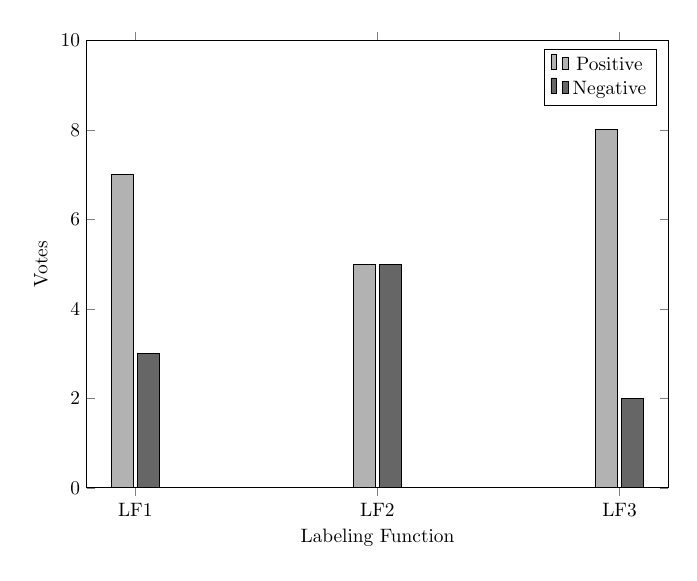
\begin{tikzpicture}[scale=0.7]
    \begin{axis}[
        ybar,
        xlabel={Labeling Function},
        ylabel={Votes},
        ymin=0, ymax=10,
        xtick={1,2,3},
        xticklabels={LF1, LF2, LF3},
        width=\textwidth,
        height=0.8\textwidth,
        bar width=0.4cm,
    ]
    \addplot[fill=black!30] coordinates {(1,7) (2,5) (3,8)};
    \addplot[fill=black!60] coordinates {(1,3) (2,5) (3,2)};
    \legend{Positive, Negative}
    \end{axis}
\end{tikzpicture}
\caption{Three labelling functions voting on examples. They disagree.}
\label{fig:lf_votes}
\end{marginfigure}

You want to classify emails as spam or not-spam. You write three rules:
\begin{enumerate}
    \item LF1: Contains ``free money'' $\to$ spam
    \item LF2: From known contact $\to$ not spam
    \item LF3: Contains link + urgency words $\to$ spam
\end{enumerate}

For an email from a known contact about a ``free trial offer'':
\begin{itemize}
    \item LF1 votes: spam, matches ``free''
    \item LF2 votes: not spam, known contact
    \item LF3 votes: abstain, no link
\end{itemize}

How do you combine these conflicting votes?

\newthought{The Learning Objectives} of this lecture:
\begin{itemize}
    \item Design labelling functions that encode domain knowledge and characterise their coverage-accuracy trade-off.
    \item Apply the Snorkel framework to aggregate noisy label sources into probabilistic training labels via a learned label model.
    \item Handle remaining label noise through loss correction, sample weighting, and co-teaching.
\end{itemize}

%═══════════════════════════════════════════════════════════════════════
% BLOCK 2: MAIN THEORY
%═══════════════════════════════════════════════════════════════════════

\newpage
\section{Sources of Weak Labels}\index{weak labels}

\marginnote{Weak labels come from many sources, each with different characteristics.}

\begin{table}
\centering
\begin{tabular}{lcc}
\toprule
\textbf{Source} & \textbf{Coverage} & \textbf{Accuracy} \\
\midrule
Expert annotation & High & High (95\%+) \\
Crowd workers & High & Medium (70--90\%) \\
Heuristic rules & Low--Medium & Variable \\
Distant supervision & High & Low--Medium \\
Pre-trained models & High & Medium--High \\
\bottomrule
\end{tabular}
\caption{Common weak supervision sources.}
\label{tab:weak_sources}
\end{table}

\newthought{Noisy crowd labels} come from multiple annotators with varying quality. Distant supervision\index{distant supervision} derives labels from knowledge bases, for example labelling all sentences mentioning two entities in a relation as expressing that relation. Heuristic rules encode domain knowledge as functions. Data augmentation lets transformed examples inherit parent labels. Auxiliary signals such as metadata, user behaviour, and sensor data provide additional evidence.


\section{Labeling Functions}\index{labeling function}

\marginnote{A labelling function is a noisy voter that may abstain.}

\newthought{A labelling function} $\lambda: X \to Y \cup \{\emptyset\}$ maps inputs to a label or abstention $\emptyset$.

\newthought{Examples for text classification:}
\begin{itemize}
    \item Keyword matching: contains(``urgent'') $\to$ spam
    \item Pattern matching: regex for phone numbers $\to$ contact info
    \item External models: sentiment classifier output
    \item Heuristics: short emails $\to$ not spam
\end{itemize}

\subsection{Properties of Good Labeling Functions}

\newthought{Good labelling functions} have high precision, so that when they vote they are usually right; reasonable coverage, so that they vote on enough examples; diversity, so that different LFs capture different patterns; and low correlation, so that their errors are independent.

\begin{figure}
\centering
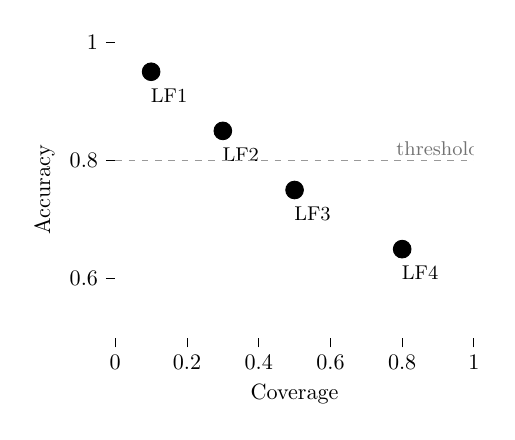
\begin{tikzpicture}[scale=0.8]
    \begin{axis}[
        xlabel={Coverage},
        ylabel={Accuracy},
        xmin=0, xmax=1,
        ymin=0.5, ymax=1,
        width=0.6\textwidth,
        axis line style={draw=none},
        tick style={black, thin},
        tick align=outside, tick pos=left,
    ]
    \addplot[only marks, mark=*, mark size=4pt] coordinates {
        (0.1, 0.95) (0.3, 0.85) (0.5, 0.75) (0.8, 0.65)
    };
    \node at (axis cs:0.15, 0.91) {\small LF1};
    \node at (axis cs:0.35, 0.81) {\small LF2};
    \node at (axis cs:0.55, 0.71) {\small LF3};
    \node at (axis cs:0.85, 0.61) {\small LF4};
    \draw[dashed, black!40] (axis cs:0,0.8) -- (axis cs:1,0.8);
    \node[black!55] at (axis cs:0.9, 0.82) {\small threshold};
    \end{axis}
\end{tikzpicture}
\caption{Labelling functions trade off coverage and accuracy.}
\label{fig:lf_tradeoff}
\end{figure}


\section{Label Modeling}\index{label model}

\marginnote{The label model estimates true labels from noisy votes.}

\subsection{Majority Vote}

\newthought{The simplest aggregation} is majority vote:
\begin{equation}
    \hat{y} = \text{mode}(\{\lambda_i(x) : \lambda_i(x) \neq \emptyset\})
\end{equation}

This assumes equal accuracy and ignores correlations.

\subsection{Modeling Labeler Accuracy}

\newthought{Treating each LF} as having accuracy $\alpha_i = P(\lambda_i(x) = y | \lambda_i(x) \neq \emptyset)$ gives a weighted vote:

\begin{equation}
    P(y | \lambda_1, \ldots, \lambda_m) \propto P(y) \prod_{i: \lambda_i \neq \emptyset} P(\lambda_i | y)
\end{equation}

\subsection{Modeling Correlations}

\newthought{Labelling functions may have correlated errors,} for example two keyword-based LFs that fail on the same examples.

A factor graph model captures pairwise correlations:
\begin{equation}
    P(y, \lambda_1, \ldots, \lambda_m) = \frac{1}{Z} \phi_Y(y) \prod_i \phi_i(y, \lambda_i) \prod_{i,j} \phi_{ij}(\lambda_i, \lambda_j)
\end{equation}

where $\phi_{ij}$ captures the pairwise dependency structure.


\section{The Snorkel Framework}\index{Snorkel}

\marginnote{\newthought{Snorkel.} End-to-end weak supervision system~\cite{Ratner2017Snorkel}.}

\begin{figure}
\centering
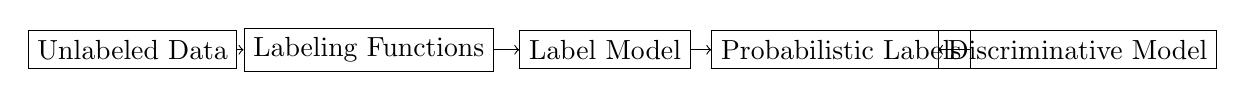
\begin{tikzpicture}[node distance=1.5cm]
    \node[draw, rectangle] (data) {Unlabeled Data};
    \node[draw, rectangle, right of=data, xshift=1.5cm] (lfs) {Labeling Functions};
    \node[draw, rectangle, right of=lfs, xshift=1.5cm] (lm) {Label Model};
    \node[draw, rectangle, right of=lm, xshift=1.5cm] (prob) {Probabilistic Labels};
    \node[draw, rectangle, right of=prob, xshift=1.5cm] (dm) {Discriminative Model};

    \draw[->] (data) -- (lfs);
    \draw[->] (lfs) -- (lm);
    \draw[->] (lm) -- (prob);
    \draw[->] (prob) -- (dm);
\end{tikzpicture}
\caption{Snorkel pipeline: LFs $\to$ Label Model $\to$ Probabilistic Labels $\to$ Train End Model.}
\label{fig:snorkel_pipeline}
\end{figure}

\begin{algorithm}[H]
\caption{Snorkel Workflow}
\begin{algorithmic}[1]
\State \textbf{Write} labeling functions encoding domain knowledge
\State \textbf{Apply} LFs to unlabeled data $\to$ label matrix $\Lambda$
\State \textbf{Train} label model on $\Lambda$ to estimate LF accuracies and correlations
\State \textbf{Generate} probabilistic labels $\tilde{y} = P(y | \Lambda)$
\State \textbf{Train} discriminative model on $(X, \tilde{y})$
\end{algorithmic}
\end{algorithm}

\newthought{The key insight} is that the discriminative model generalises beyond the labelling functions; it learns features, not just rules.


\section{Learning with Label Noise}\index{label noise}

\marginnote{Even with probabilistic labels, training can be noisy.}

\subsection{Forward and Backward Loss Correction}

\newthought{If noise is class-conditional} with known transition matrix $T$ where $T_{ij} = P(\tilde{y} = j | y = i)$:

Forward correction:
\begin{equation}
    \tilde{\ell}(f(x), \tilde{y}) = \ell(f(x), T^T f(x))
\end{equation}

Backward correction:
\begin{equation}
    \tilde{\ell}(f(x), \tilde{y}) = T^{-1} \ell(f(x), \tilde{y})
\end{equation}

\subsection{Sample Weighting}

\newthought{Down-weighting likely-mislabelled examples} gives:
\begin{equation}
    \mathcal{L} = \sum_i w_i \ell(f(x_i), \tilde{y}_i)
\end{equation}

where $w_i$ is based on loss value, prediction confidence, or label model confidence.

\subsection{Co-Teaching}\index{co-teaching}

\newthought{Co-teaching} trains two networks~\cite{Han2018CoTeaching}; each selects small-loss samples for the other:
\begin{itemize}
    \item Network A selects clean samples for Network B
    \item Network B selects clean samples for Network A
    \item Both avoid memorising the same noisy labels
\end{itemize}


\section{Active Learning}\index{active learning}

\marginnote{\newthought{Weak supervision} works with the labels you already have. Active learning chooses which labels to request next.}

\newthought{Labelling functions are cheap, but human time is not.} An expert can produce a near-perfect label for any single example, yet their throughput is bounded; in industrial settings the oracle is rate limited by contract or by attention. Active learning\index{active learning}~\cite{Settles2012ActiveLearning} accepts this constraint and asks a different question, namely which input, if labelled now, would most improve the model.

\newthought{Where weak supervision combined many noisy votes,} active learning escalates a single example to a clean vote. The two are complementary; they sit on the same axis of imperfect supervision but pull in opposite directions. Snorkel asks how to make do with what we have. Active learning asks what to ask for next.

\newthought{The acquisition function} formalises this choice. Given a pool of unlabelled inputs $\mathcal{U}$ and a budget of $b$ queries, we score every $x \in \mathcal{U}$ by an informativeness function $a(x)$ and request labels for the top-$b$ examples. Different definitions of $a$ produce different querying behaviours.

\subsection{Uncertainty Sampling}\index{uncertainty sampling}

\marginnote{\newthought{Callback to chapter 7.} The predictive entropy and the margin we used for routing-to-human now drive what we ask the human about.}

\newthought{Uncertainty sampling} picks the input where the model is least sure of its prediction. The predictive entropy
\begin{equation}
    a_{\text{ent}}(x) = -\sum_y p_\theta(y \mid x) \log p_\theta(y \mid x)
\end{equation}
peaks when the softmax distribution is flat. The margin
\begin{equation}
    a_{\text{mar}}(x) = -\bigl(p_\theta(y_1^* \mid x) - p_\theta(y_2^* \mid x)\bigr)
\end{equation}
focuses on the gap between the top two classes; small margins flag near-tie decisions. Both are direct consumers of the calibrated probabilities from chapter 7, which is what makes the uncertainty machinery so reusable here.

\subsection{Query by Committee}\index{query by committee}

\newthought{Query by committee} replaces a single model with an ensemble and queries inputs where ensemble members disagree most. Disagreement can be measured by vote entropy across the committee or by the average KL divergence between each member's predictive distribution and the ensemble mean. Deep ensembles\index{deep ensembles}~\cite{Lakshminarayanan2017} provide a clean implementation; MC Dropout from chapter 7 is the cheap stand-in when training $M$ networks is too expensive.

\newthought{Disagreement is structurally different from uncertainty.} A single overconfident model can be confidently wrong; an ensemble of models trained from different seeds will spread their probability mass on inputs the data did not pin down. Query by committee therefore catches epistemic uncertainty that uncertainty sampling on a single model can miss.

\subsection{Expected Model Change}\index{expected model change}

\newthought{Expected model change} flips the question. Rather than asking where the model is unsure, it asks which label would shift the parameters the most. A common surrogate is the expected gradient length,
\begin{equation}
    a_{\text{egl}}(x) = \mathbb{E}_{y \sim p_\theta(y \mid x)} \bigl\| \nabla_\theta \mathcal{L}(x, y) \bigr\|.
\end{equation}
The label is hypothetical, so the expectation runs over the model's current belief. This is principled, since it directly targets parameter movement, but it is also expensive; every candidate requires a gradient evaluation per possible label. In practice it is reserved for small pools or for selecting batches in the final rounds where uncertainty has plateaued.

\subsection{Pool, Stream, and Membership Query}\index{pool-based active learning}

\newthought{The setting changes the algorithm.} In pool-based active learning the entire unlabelled set $\mathcal{U}$ sits on disk and we score every example before each query round; this is the standard text or image setup. In stream-based selective sampling the inputs arrive one at a time and we must decide on the spot whether to forward this one to the oracle, common in network monitoring and click streams. In membership query synthesis the learner constructs a synthetic input and asks the oracle to label it, which is powerful but often produces inputs no human can interpret. Pool-based is the default for the rest of this section.

\subsection{The Cold-Start Problem}\index{cold start}

\marginnote{\newthought{Cold start} is why every active-learning pipeline opens with a small random or stratified seed before the acquisition function takes over.}

\newthought{Active learning has a chicken-and-egg flaw} at the start. The acquisition functions above all rely on the model's own probabilities or its own gradient. With ten labels and a freshly initialised network those probabilities are nearly uniform, so the entropy is high everywhere and the model points the oracle at random points. Worse, the calibration tools from chapter 7 also need data; an underfit model is overconfident on the training set and uniformly confused off it.

\newthought{The fix is a clean seed.} A small batch of labels chosen by stratified random sampling, or by clustering on representations and picking medoids, gives the model enough signal to produce uncertainty estimates that mean something. Only then is it safe to switch over to uncertainty sampling or query by committee. Treat the first few rounds as bootstrap, not as exploitation.

\subsection{Composition with Weak Supervision}

\newthought{Active learning and weak supervision compose} into a hybrid pipeline that uses each for what it does well. The model fits on the probabilistic labels from Snorkel; the acquisition function flags the inputs where Snorkel and the model disagree, or where the label model itself is uncertain because too few labelling functions voted. The oracle then labels those inputs, but the human is not asked only for a label; they are asked why, and the why becomes a new labelling function. The model's uncertainty signal therefore drives both the next label request and the next labelling-function priority, closing a loop between cheap programmatic supervision and expensive human supervision.

\begin{figure}
\centering
\begin{tikzpicture}[
    node distance=1.4cm,
    every node/.style={font=\small, align=center},
    block/.style={rectangle, draw=black, thick, rounded corners=2pt,
                  minimum width=2.4cm, minimum height=0.7cm, inner sep=4pt},
    arr/.style={-{Triangle[length=4pt, width=4pt, fill=black!70]}, thick, black!70},
]
    \node[block] (pool) {Unlabelled Pool $\mathcal{U}$};
    \node[block, right=of pool] (acq) {Acquisition $a(x)$};
    \node[block, right=of acq] (oracle) {Oracle};
    \node[block, below=of acq, fill=black!8] (model) {Model $p_\theta$};
    \draw[arr] (pool.east) -- (acq.west);
    \draw[arr] (acq.east) -- (oracle.west);
    \draw[arr] (oracle.south) |- node[right, font=\tiny, pos=0.25] {labelled $(x, y)$} (model.east);
    \draw[arr] (model.west) -| node[left, font=\tiny, pos=0.75] {$p_\theta(y \mid x)$} (acq.south);
\end{tikzpicture}
\caption{The active-learning loop. The model's predictive distribution feeds the acquisition function, which selects inputs from the pool for the oracle, whose labels retrain the model.}
\label{fig:active_learning_loop}
\end{figure}

\newthought{Notice that the acquisition function} is the only place where chapter 7 and chapter 10 actually meet. Predictive entropy was a routing signal there; it is a query signal here. Same number, different downstream consumer.


\section{Association Rules as Labeling Functions}\index{association rules}

\marginnote{From Apriori to labelling: mine rules from data structure.}

\newthought{Association rule learning} and labelling functions share a common structure: association rules $\{A, B\} \to \{C\}$ are scored by support and confidence, while labelling functions map $\text{condition}(x) \to \text{label}$.

Mining frequent patterns can automatically generate labelling functions:
\begin{enumerate}
    \item Find frequent itemsets in feature space
    \item Convert to rules with confidence threshold
    \item Use as labelling functions
\end{enumerate}


%═══════════════════════════════════════════════════════════════════════
% BLOCK 3: STUDENT ACTIVATION
%═══════════════════════════════════════════════════════════════════════

\newpage
\section{Examples \& Exercises}

\subsection{Exercise 1: Write Labeling Functions}

Design 5 labelling functions for classifying product reviews as positive or negative.

\subsection{Exercise 2: Label Aggregation}

Three LFs vote on an example:
\begin{itemize}
    \item LF1: positive, accuracy 0.9
    \item LF2: negative, accuracy 0.8
    \item LF3: positive, accuracy 0.7
\end{itemize}

Assuming independent LFs and uniform prior, compute $P(y = \text{positive})$.

\subsection{Exercise 3: LF Correlation}

Two LFs both use keyword matching. Why might their errors be correlated? How does this affect the label model?

\subsection{Exercise 4: Acquisition Function Bake-Off}

A three-class classifier returns the following softmax probabilities over $\{c_1, c_2, c_3\}$ on six pool inputs:

\begin{table*}[ht]
\centering
\begin{tabular}{p{0.10\textwidth}p{0.12\textwidth}p{0.12\textwidth}p{0.12\textwidth}}
    \toprule
    \textbf{Input} & \textbf{$p(c_1)$} & \textbf{$p(c_2)$} & \textbf{$p(c_3)$} \\
    \midrule
    $u_1$ & $0.80$ & $0.15$ & $0.05$ \\
    $u_2$ & $0.45$ & $0.40$ & $0.15$ \\
    $u_3$ & $0.34$ & $0.33$ & $0.33$ \\
    $u_4$ & $0.60$ & $0.30$ & $0.10$ \\
    $u_5$ & $0.50$ & $0.45$ & $0.05$ \\
    $u_6$ & $0.95$ & $0.04$ & $0.01$ \\
    \bottomrule
\end{tabular}
\vspace{2em}
\caption{Predicted softmax distributions for six pool inputs. Each row sums to one.}
\label{tab:al_pool}
\end{table*}

Your tasks: compute the predictive entropy and the margin for every input, then identify the top-2 queries that uncertainty sampling and margin sampling would each request. Comment on whether they agree.

\vspace{0.5em}

\newthought{Step.} For $u_2$, the entropy is
\begin{align*}
    a_{\text{ent}}(u_2) &= -\bigl(0.45 \log 0.45 + 0.40 \log 0.40 + 0.15 \log 0.15\bigr) \\
                        &\approx 0.359 + 0.366 + 0.285 \\
                        &\approx 1.010 \text{ nats}
\end{align*}
and the margin is $a_{\text{mar}}(u_2) = -(0.45 - 0.40) = -0.05$. Repeat for the other five inputs and rank them.

\newthought{Reflect.} Suppose you also have a deep ensemble of three models that all return the same row for $u_3$ but disagree sharply on $u_5$. Which input would query by committee prefer, and why does this differ from what the single-model entropy says?


\section{Self-Reflection and Recap}

\newthought{Self-Reflection.}

\begin{enumerate}
    \item When is weak supervision preferable to collecting clean labels?
    \item How do you know if your labelling functions are good enough?
    \item What happens to the label model when all labelling functions are correlated?
    \item Why does the discriminative model in Snorkel generalise beyond the labelling functions themselves?
    \item How does co-teaching avoid the confirmation bias that a single network would accumulate?
    \item What are the risks of distant supervision, and how would you mitigate them?
    \item Could you combine weak supervision with active learning, and if so, how?
    \item Why is uncertainty sampling unsafe in the very first round of active learning, and what should you do instead?
    \item When would you prefer query by committee over single-model uncertainty sampling, and what does that say about the kind of uncertainty each strategy captures?
\end{enumerate}

\vspace{1.5em}

\newthought{Recap.}

\begin{itemize}
    \item Weak supervision embraces label noise by modelling labeller accuracy and correlation rather than treating annotations as ground truth.
    \item Labelling functions encode domain knowledge as noisy voters; the coverage-accuracy trade-off determines their utility in the label model.
    \item Snorkel aggregates multiple noisy sources into probabilistic labels and trains a discriminative model that generalises beyond the rules.
    \item Noise-robust training via loss correction, sample weighting, and co-teaching handles residual label errors after aggregation.
    \item Active learning chooses which unlabelled inputs to escalate to a human oracle by scoring them with an acquisition function such as predictive entropy, margin, ensemble disagreement, or expected gradient length.
    \item Active learning and weak supervision compose; the model's uncertainty signal both prioritises label requests and surfaces gaps that the next labelling function should cover, but the cold-start problem forces a clean seed before any acquisition function can be trusted.
\end{itemize}

\vspace{2.5em}

\marginnote{\newthought{Root cause.} Every method in this chapter assumed the human only ever delivers a class label, never a behaviour or a correction.}

\newthought{The oracle in this chapter was a labelling oracle.} A medical-triage classifier trained with Snorkel and refined by uncertainty sampling can ask the radiologist whether a lesion is benign or malignant, but it cannot ask the radiologist how she would have moved the probe, nor can it watch her decide when to stop scanning. For sequential tasks, robotic manipulation, dialogue, surgical assistance, the informative supervision is not a label on a single input but a trajectory of decisions across time. A label-only oracle cannot transmit that.

\newthought{Interactive and imitation learning broaden the oracle.} Rather than querying for a label, the next chapter queries for a demonstration, a correction, or a reward. Active learning and weak supervision generalise here in the obvious way; the acquisition function still picks the most informative state to ask about, but what comes back is an action sequence, not a class. The cold-start problem reappears in a sharper form, because covariate shift means a partly trained imitator drifts into states the demonstrator never visited.

\marginnote{\newthought{Teaser.} If the oracle no longer hands you a label but takes the wheel, what exactly are you learning?}

\newthought{The next chapter explores interactive and imitation learning,} where behaviour cloning, DAgger-style correction, and inverse reinforcement learning extend the active-learning idea from labels to whole policies.

\marginnote{\newthought{feedback}}
